
%%%%%%%%%%%%%%%%%%%%%%%%%%%%%%%%%%%%%%%%%%%%%%%%%%%%%%%%%%%%%%%%%%%%%%%%%%%%%%
% Copyright (c) 2003-2016 by The University of Queensland
% http://www.uq.edu.au
%
% Primary Business: Queensland, Australia
% Licensed under the Apache License, version 2.0
% http://www.apache.org/licenses/LICENSE-2.0
%
% Development until 2012 by Earth Systems Science Computational Center (ESSCC)
% Development 2012-2013 by School of Earth Sciences
% Development from 2014 by Centre for Geoscience Computing (GeoComp)
%
%%%%%%%%%%%%%%%%%%%%%%%%%%%%%%%%%%%%%%%%%%%%%%%%%%%%%%%%%%%%%%%%%%%%%%%%%%%%%%

\section{Elastic Deformation}
\label{ELASTIC CHAP}
In this section we want to examine the deformation of a linear elastic body caused by expansion through a heat distribution.
We want a displacement field $u_{i}$ which solves the momentum
equation\index{momentum equation}:
\begin{eqnarray}\label{HEATEDBLOCK general problem}
 - \sigma_{ij,j}=0
\end{eqnarray}
where the stress $\sigma$ is given by
\begin{eqnarray}\label{HEATEDBLOCK linear elastic}
 \sigma_{ij}= \lambda u_{k,k} \delta_{ij} + \mu ( u_{i,j} + u_{j,i})
 - (\lambda+\frac{2}{3} \mu)  \; \alpha  \;  (T-T_{ref})\delta_{ij} \;.
\end{eqnarray}
In this formula $\lambda$ and $\mu$ are the Lam\'e coefficients, $\alpha$ is the
temperature expansion coefficient, $T$ is the temperature distribution and $T_{ref}$ a reference temperature.
Note that \eqn{HEATEDBLOCK general problem} is similar to \eqn{WAVE general problem}
introduced in \Sec{WAVE CHAP} but the inertia term $\rho u_{i,tt}$
has been dropped as we assume a static scenario here.
Moreover, in comparison to the \eqn{WAVE stress} definition of stress $\sigma$
in \eqn{HEATEDBLOCK linear elastic} an extra term is introduced to bring in
stress due to volume changes through temperature dependent expansion.

Our domain is the unit cube
\begin{eqnarray} \label{HEATEDBLOCK natural location}
\Omega=\{(x_{i}) | 0 \le x_{i} \le 1 \}
\end{eqnarray}
On the boundary the normal stress component is set to zero
\begin{eqnarray} \label{HEATEDBLOCK natural}
\sigma_{ij}n_{j}=0
\end{eqnarray}
and on the face with $x_{i}=0$ we set the $i$-th component of the displacement to $0$:
\begin{eqnarray} \label{HEATEDBLOCK constraint}
u_{i}(x)=0 & \mbox{ where } & x_{i}=0 \;
\end{eqnarray}
For the temperature distribution we use
\begin{eqnarray} \label{HEATEDBLOCK temperature}
T(x)= T_{0} e^{-\beta \|x-x^{c}\|}
\end{eqnarray}
with a given positive constant $\beta$ and location $x^{c}$ in the domain.

%Later in \Sec{MODELFRAME} we will use
% $T$ from a time-dependent temperature diffusion problem as discussed in \Sec{DIFFUSION CHAP}.
When we insert \eqn{HEATEDBLOCK linear elastic} we get a second order system
of linear PDEs for the displacements $u$ which is called the Lam\'e equation\index{Lam\'e equation}.
We want to solve this using the \LinearPDE class.
For a system of PDEs and a solution with several components the \LinearPDE class takes PDEs of the form
\begin{equation}\label{LINEARPDE.SYSTEM.1 TUTORIAL}
-(A_{ijkl} u_{k,l})_{,j}=-X_{ij,j} \; .
\end{equation}
$A$ is a \RankFour and $X$ is a \RankTwo.
We show here the coefficients relevant for the problem we are trying to solve.
The full form is given in \eqn{LINEARPDE.SYSTEM.1}.
The natural boundary conditions\index{boundary condition!natural} take the form
\begin{equation}\label{LINEARPDE.SYSTEM.2 TUTORIAL}
n_{j} A_{ijkl} u_{k,l}=n_{j}X_{ij}
\end{equation}
while constraints\index{constraint} take the form
\begin{equation}\label{LINEARPDE.SYSTEM.3 TUTORIAL}
u_{i}=r_{i} \mbox{ where } q_{i}>0
\end{equation}
$r$ and $q$ are each a \RankOne.
We can easily identify the coefficients in \eqn{LINEARPDE.SYSTEM.1 TUTORIAL}:
\begin{eqnarray}\label{LINEARPDE ELASTIC COEFFICIENTS}
A_{ijkl}=\lambda \delta_{ij} \delta_{kl} + \mu (
\delta_{ik} \delta_{jl}
+ \delta_{il} \delta_{jk}) \\
X_{ij}=(\lambda+\frac{2}{3} \mu) \;  \alpha \; (T-T_{ref})\delta_{ij} \\
\end{eqnarray}
The characteristic function $q$ defining the locations and components where constraints are set is given by:
\begin{equation}\label{HEATEDBLOCK MASK}
q_{i}(x)=\left\{
\begin{array}{cl}
1 & x_{i}=0\\
0 & \mbox{otherwise.}\\
\end{array}
\right.
\end{equation}
Under the assumption that $\lambda$, $\mu$, $\beta$ and $T_{ref}$
are constant we may use $Y_{i}=(\lambda+\frac{2}{3} \mu) \; \alpha \; T_{i}$.
However, this choice would lead to a different natural boundary condition
which does not set the normal stress component as defined in \eqn{HEATEDBLOCK linear elastic} to zero.

Analogous to the concept of symmetry for a single PDE, we call the PDE
defined by \eqn{LINEARPDE.SYSTEM.1 TUTORIAL} symmetric\index{symmetric PDE} if
\begin{eqnarray}\label{LINEARPDE.SYSTEM.SYMMETRY TUTORIAL}
A_{ijkl} =A_{klij} \\
\end{eqnarray}
This Lam\'e equation is in fact symmetric, given the difference in $D$ and $d$ as compared to the scalar case.
The \LinearPDE class is notified of this fact by calling its \method{setSymmetryOn} method.

After we have solved the Lam\'e equation we want to analyse the actual stress distribution.
Typically the \emph{von-Mises} stress\index{von-Mises stress} defined by
\begin{equation}
\sigma_{mises} = \sqrt{
\frac{1}{2} ((\sigma_{00}-\sigma_{11})^2
            + (\sigma_{11}-\sigma_{22})^2
            + (\sigma_{22}-\sigma_{00})^2)
+ 3( \sigma_{01}^2+\sigma_{12}^2+\sigma_{20}^2) }
\end{equation}
is used to detect material damage.
Here we want to calculate the von-Mises stress and write it to a file for visualization.

The following script, which is available in \file{heatedblock.py} in the
\ExampleDirectory, solves the Lam\'e equation and writes the displacements and
the von-Mises stress\index{von-Mises stress} into a file \file{deform.vtu} in
the \VTK file format\index{scripts!\file{diffusion.py}}:
\begin{python}
  from esys.escript import *
  from esys.escript.linearPDEs import LinearPDE
  from esys.finley import Brick
  from esys.weipa import saveVTK
  #... set some parameters ...
  lam=1.
  mu=0.1
  alpha=1.e-6
  xc=[0.3, 0.3, 1.]
  beta=8.
  T_ref=0.
  T_0=1.
  #... generate domain ...
  mydomain = Brick(l0=1., l1=1., l2=1., n0=10, n1=10, n2=10)
  x=mydomain.getX()
  #... set temperature ...
  T=T_0*exp(-beta*length(x-xc))
  #... open symmetric PDE ...
  mypde=LinearPDE(mydomain)
  mypde.setSymmetryOn()
  #... set coefficients ...
  C=Tensor4(0., Function(mydomain))
  for i in range(mydomain.getDim()):
    for j in range(mydomain.getDim()):
       C[i,i,j,j]+=lam
       C[i,j,i,j]+=mu
       C[i,j,j,i]+=mu
  msk=whereZero(x[0])*[1.,0.,0.] \
     +whereZero(x[1])*[0.,1.,0.] \
     +whereZero(x[2])*[0.,0.,1.]
  sigma0=(lam+2./3.*mu)*alpha*(T-T_ref)*kronecker(mydomain)
  mypde.setValue(A=C, X=sigma0, q=msk)
  #... solve pde ...
  u=mypde.getSolution()
  #... calculate von-Mises stress
  g=grad(u)
  sigma=mu*(g+transpose(g))+lam*trace(g)*kronecker(mydomain)-sigma0
  sigma_mises=sqrt(((sigma[0,0]-sigma[1,1])**2+(sigma[1,1]-sigma[2,2])**2+ \
                    (sigma[2,2]-sigma[0,0])**2)/2. \
                   +3*(sigma[0,1]**2 + sigma[1,2]**2 + sigma[2,0]**2))
  #... output ...
  saveVTK("deform.vtu", disp=u, stress=sigma_mises)
\end{python}

\begin{figure}
\centerline{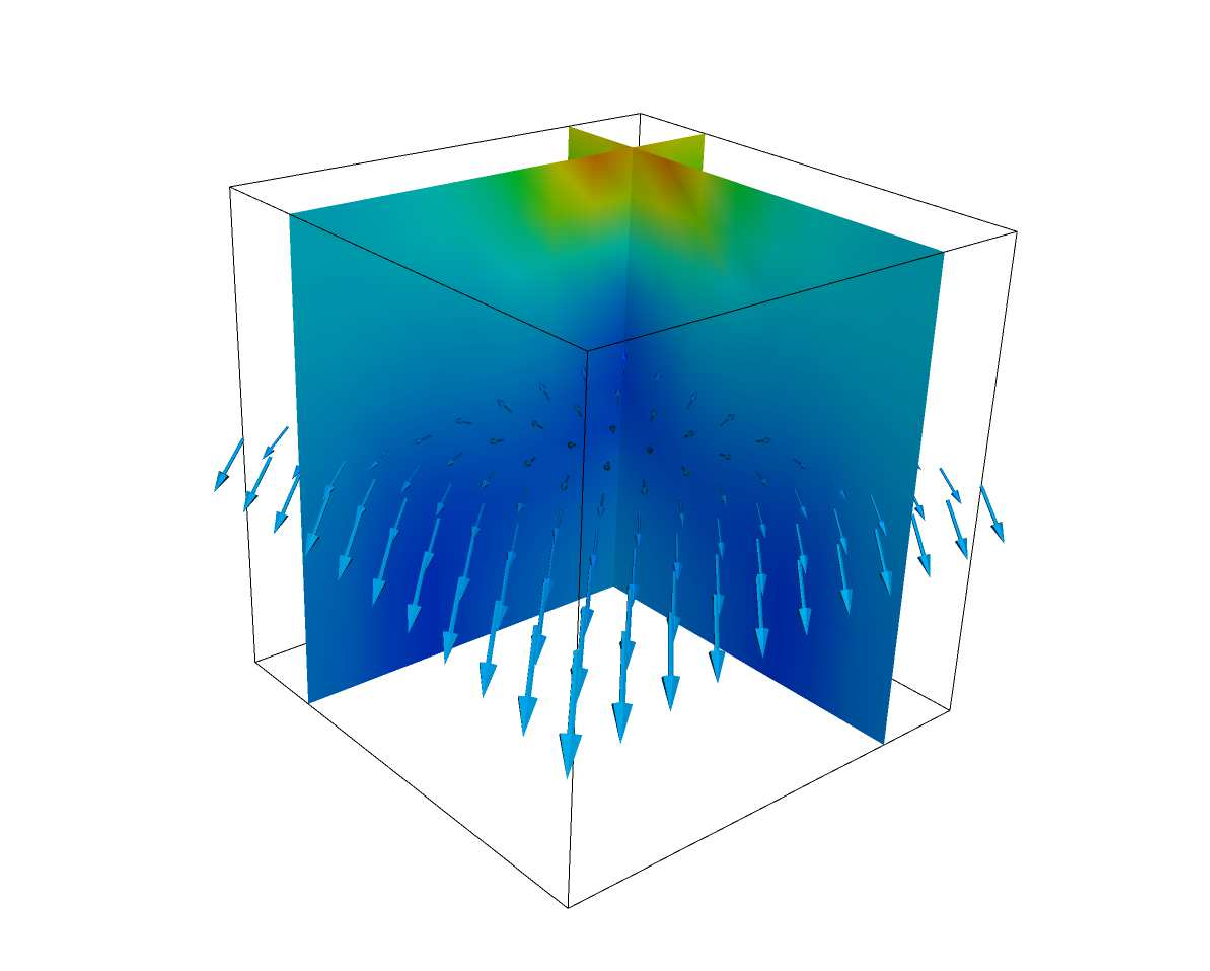
\includegraphics[width=\figwidth]{HeatedBlock}}
\caption{von-Mises Stress and Displacement Vectors}
\label{HEATEDBLOCK FIG 2}
\end{figure}

\noindent Finally, the results can be visualized by calling
\begin{verbatim}
mayavi2 -d deform.vtu -f CellToPointData -m Vectors -m Surface
\end{verbatim}
Note that the filter \text{CellToPointData} is applied to create a smoother
representation of the von-Mises stress.
\fig{HEATEDBLOCK FIG 2} shows the results where the colour of the vertical
planes represent the von-Mises stress and a horizontal plane of arrows shows
the displacements vectors.

